\documentclass[11pt]{article}

\usepackage{mathptmx}
\usepackage{url}
\usepackage{graphicx}

\newcommand*{\p}[1]{\textup{\texttt{#1}}}
\newcommand*{\ls}{\textsc{LearnSAT}}
\newcommand*{\pl}{\textsc{Prolog}}
\newcommand*{\sw}{\textsc{SWI-Prolog}}
\newcommand*{\dt}{\textsc{dot}}

\textwidth=16cm
\textheight=22cm
\topmargin=0pt
\headheight=0pt
\oddsidemargin=5mm
\headsep=0pt
\renewcommand{\baselinestretch}{1.1}
\setlength{\parskip}{0.20\baselineskip plus 1pt minus 1pt}
\parindent=0pt

\title{\bfseries \ls{} --- User's Guide\\\mbox{}\\\mbox{}\\
\bfseries\normalsize Version 1.4.1}

\author{\bfseries Mordechai (Moti) Ben-Ari\\\mbox{}\\
\url{http: //www.weizmann.ac.il/sci-tea/benari/}}

\begin{document}

\maketitle

\thispagestyle{empty}

\vspace*{\fill}

\begin{center}
\copyright{} 2012-13 by Mordechai (Moti) Ben-Ari.
\end{center}
This work is licensed under the Creative Commons Attribution-ShareAlike 3.0
License. To view a copy of this license, visit
\url{http://creativecommons.org/licenses/by-sa/3.0/}; or, (b) send a letter
to Creative Commons, 543 Howard Street, 5th Floor, San Francisco,
California, 94105, USA.

\bigskip\bigskip

 
\begin{center}
The following copyright notice applies to the programs described in this
document:\mbox{}\\\mbox{}\\
\copyright{} 2012-13 by Mordechai (Moti) Ben-Ari.
\end{center}

This program is free software; you can redistribute it and/or
modify it under the terms of the GNU General Public License
as published by the Free Software Foundation; either version 2
of the License, or (at your option) any later version.
This program is distributed in the hope that it will be useful
but WITHOUT ANY WARRANTY; without even the implied warranty of
MERCHANTABILITY or FITNESS FOR A PARTICULAR PURPOSE.
See the GNU General Public License for more details.
You should have received a copy of the GNU General Public License
along with this program; if not, write to the Free Software
Foundation, Inc., 59 Temple Place - Suite 330, Boston, MA
02111-1307, USA.

\setcounter{page}{0}
\newpage

\section{Overview}

\ls{} is a program for learning about SAT solving. It implements the
classic \emph{Davis-Putnam-Logemann-Loveland (DPLL)} algorithm, together
with modern extensions of the algorithm: \emph{conflict-driven clause
learning (CDCL)} and \emph{non-chronological backtracking (NCB)}.

For a gentle introduction to SAT solvers, see \cite[Chapter~6]{mlcs}.
The comprehensive reference is the \emph{Handbook of Satisfiability}
\cite{SAT}. The algorithms and notation of \ls{} follow \cite{mlm}.

The design of \ls{} is based on the following principles:

\begin{itemize}

\item A trace of the algorithm's execution is
displayed. The content of the trace can be set by the user.

\item Graphical representations of implication graphs and assignment
trees are generated automatically.

\item The implementation is in \pl{} so that the program will be concise
and easy to understand.

\item \ls{} is an open-source project.

\item The software is easy to install and use.
\end{itemize}

This document contains the \emph{user's guide} and the \emph{software
documentation}.

A \emph{tutorial} on SAT solving with \ls{} can be downloaded separately.

\section{Installation}

\ls{} can be found on Google Code:
\begin{center}
\url{http://code.google.com/p/mlcs/}.
\end{center}

Download and unzip the archive \p{learnsat-N.zip}. The \pl{} source code
is in the directory \p{src} and the documentation is in the directory
\p{docs}.

Download and install \sw{}:\footnote{For possible portability problems,
see Section~\ref{s.port}.}
\begin{center}
\url{http://www.swi-prolog.org/}.
\end{center}
There are binary distributions of \sw{} for Windows and MacOSX.

The source files use the extension \p{pro} instead of the more usual
\p{pl} to avoid conflict with programs in Perl. During the installation
of \sw{}, if you associate the extension \p{pro} with \sw{}, a
program can be launched by double-clicking on its name in a file list. 

\newpage

\section{Running \ls}

The main module is in the file \p{dpll.pro}. It exports the following
predicates which are the only predicates that you need to run \ls{}:

\begin{center}
\begin{tabular}{|l|l|}
\hline
\multicolumn{2}{|c|}{\textbf{\large Predicates}}\\
\hline
\p{dpll}&Run the DPLL algorithm\\
\p{usage}&Show the predicates, modes and display options \\
\p{show\_config}&Show the current mode and display options\\
\p{set\_mode}&Set the algorithmic mode\\
\p{set\_display}&Set display options\\
\p{clear\_display}&Clear display options\\
\p{set\_order}&Set variable assignment order\\
\hline
\end{tabular}
\end{center}

To check the satisfiability of a CNF formula, create a \pl{} program
that calls the predicate \p{dpll} with the clausal form of the formula
represented as a list of lists of literals.

The file with the program must be in the \p{src} directory;
alternatively, the \ls{} source files can be copied to the directory
that contains that file.

Here is a program for the pigeonhole principle for two holes and three
pigeons, where \p{pij} means that pigeon \p{i} is in hole \p{j}:

\begin{verbatim}
:- use_module(dpll).

hole2 :-
  dpll(
  [
  [p11, p12],   [p21, p22],   [p31, p32],   % Each pigeon in hole 1 or 2 
  [~p11, ~p21], [~p11, ~p31], [~p21, ~p31], % No pair is in hole 1
  [~p12, ~p22], [~p12, ~p32], [~p22, ~p32], % No pair is in hole 2
  ], _).
\end{verbatim}

The result (a satisfying assignment or \p{[]} if unsatisfiable) is
returned as the second argument, but can be left anonymous if only
the trace is of interest.

Once this file has been loaded (by double-clicking or by consulting
\p{[pigeon]}), the query:
\begin{verbatim}
?- hole2. 
\end{verbatim}
can be run. After it terminates with \p{true} you must press
return to get a new prompt.

\newpage

The output will be a trace of the DPLL algorithm:

\begin{verbatim}
1 ?- hole2.
LearnSAT v1.3.4. Copyright 2012-13 by Moti Ben-Ari. GNU GPL.
Decision assignment: p11=0
Propagate unit:  p12 (p12=1) derived from: 1. [p11,p12]
Propagate unit: ~p22 (p22=0) derived from: 7. [~p12,~p22]
Propagate unit:  p21 (p21=1) derived from: 2. [p21,p22]
Propagate unit: ~p31 (p31=0) derived from: 6. [~p21,~p31]
Propagate unit:  p32 (p32=1) derived from: 3. [p31,p32]
Conflict clause: 8. [~p12,~p32]
Decision assignment: p11=1
Propagate unit: ~p21 (p21=0) derived from: 4. [~p11,~p21]
Propagate unit:  p22 (p22=1) derived from: 2. [p21,p22]
Propagate unit: ~p31 (p31=0) derived from: 5. [~p11,~p31]
Propagate unit:  p32 (p32=1) derived from: 3. [p31,p32]
Conflict clause: 9. [~p22,~p32]
Unsatisfiable:
Statistics: clauses=9, variables=6, units=9, decisions=2, conflicts=2
true.
\end{verbatim}

The trace output can be directed to a file:

\begin{verbatim}
?- tell('hole2.txt'), hole2, told.
\end{verbatim}

\newpage

\section{Controlling the algorithm}

\subsection{Algorithmic mode}

\ls{} can run in one of three modes set by the predicate \p{set\_mode}:

\begin{center}
\begin{tabular}{|l|l|}
\hline
\multicolumn{2}{|c|}{\textbf{\large Modes}}\\
\hline
\p{dpll} & DPLL algorithm (default)\\
\p{cdcl} & DPLL with conflict-directed clause learning\\
\p{ncb} &  DPLL with CDCL and non-chronological backtracking\\
\hline
\end{tabular}
\end{center}

For the three-layer grid-pebbling problem, the statistics for the three
modes are:
\begin{verbatim}
dpll: units=74, decisions=50, conflicts=26
cdcl: units=25, decisions=14, conflicts=8
ncb:  units=17, decisions=9,  conflicts=3
\end{verbatim}

\subsection{Order of the variables}

By default, decision assignments are made in lexicographical order of
the atomic propositions. The order can be specified by using the
predicate \p{set\_order}. The list argument to \p{set\_order} must be a
permutation of the variables in the clauses.\footnote{Suggestion: First
run a program with the display option \p{variable} set; the list of
variables will be printed out in the correct syntax for \p{set\_order}.
You can now copy and paste the list, permuting the order as needed.}
Negated variables can be given; these variables are assigned 1 before
they are assigned 0.

To restore the default order run \p{set\_order(default)}.

The \p{mlm} example finds a satisfying assignment \emph{without}
conflicts if the default order is changed:

\begin{verbatim}
set_order([x1,x2,x021,x031,x3,x4,x5,x6]).
\end{verbatim}


\section{Display options}

\ls{} writes extensive trace output as it executes the algorithms. Each
line starts with a string followed by a colon to make it easy to
postprocess the output. The content of the trace is controlled using
\p{set\_display} and \p{clear\_display}. The argument to these
predicates can be \p{all} or \p{default}, or a single option or a list
of options from the following table (where * denotes the default
options):


\begin{center}
\begin{tabular}{|l|l|}
\hline
\multicolumn{2}{|c|}{\textbf{\large Display options}}\\
\hline
\p{antecedent}  &  antecedents of the implied literals\\
\p{assignment}  &  assignments that caused a conflict\\
\p{backtrack} * &  level of non-chronological backtracking\\
\p{clause}      &  clauses to be checked for satisfiability \\
\p{conflict} *  &  conflict clauses\\
\p{decision} *  &  decision assignments \\
\p{dominator}   &  computation of the dominator\\
\p{dot}         &  implication graphs (final) in dot format \\
\p{dot\_inc}    &  implication graphs (incremental) in dot format\\
\p{evaluate}    &  evaluation of clauses for an assignment\\
\p{graph}       &  implication graphs (final) in textual format \\
\p{incremental} &  implication graphs (incremental) in textual format\\
\p{label}       &  graphs and trees labeled with clauses\\
\p{learned} *   &  learned clause by resolution\\
\p{partial}     &  partial assignments so far \\
\p{resolvent} * &  resolvents created during CDCL \\
\p{result} *    &  result of the algorithm with statistics\\
\p{skipped} *   &  assignments skipped when backtracking \\
\p{sorted} *    &  assignments displayed in sorted order\\
\p{tree}        &  trees of assignments (final) in dot format\\
\p{tree\_inc}   &  trees of assignments (incremental) in dot format\\
\p{uip} *       &  unique implication points \\
\p{unit} *      &  unit clauses \\
\p{variables}   &  variables that are not assigned so far\\
\hline
\end{tabular}
\end{center}

In \p{cdcl} and \p{ncb} modes, the assignments are written together with
their levels in the format \p{p1=0@3}.

\p{antecedent} displays an implied assignment together with its
antecedent clause : \verb+p1@3/[~p1,p3]+.

If you need to change the mode and options frequently, you can write a
predicate to do so:

\begin{verbatim}
ncb_mode :-
  set_mode(ncb), 
  set_display([default, dominator, dot, label]).
\end{verbatim}

If \p{default} appears first in a list of display options, the
others options will be added to the default ones.

\newpage

\section{Implication graphs}\label{s.impl}

When a conflict clause is encountered, \ls{} generates the implication
graph. Display option \p{graph} generates a textual representation,
while \p{dot} generates a graphical representation. Display option
\p{label} displays the antecedent clauses on each edge, not just their
numbers. Display option \p{dominator} emphasized the following nodes:
the decision assignment at the current level, the dominator and
\p{kappa}.

\begin{center}
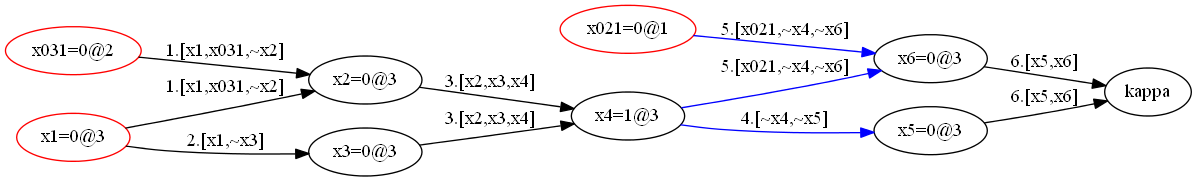
\includegraphics[keepaspectratio=true,width=.9\textwidth]{graph-color}

\bigskip

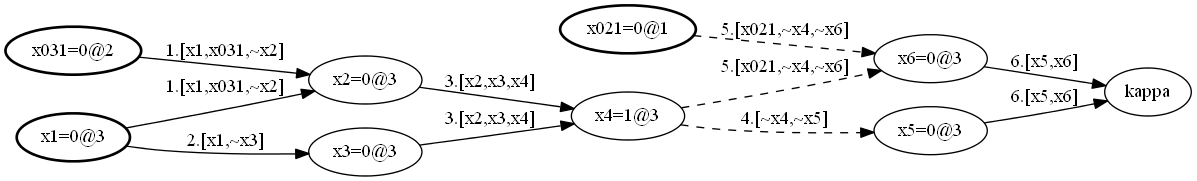
\includegraphics[keepaspectratio=true,width=.9\textwidth]{graph-bw}
\end{center}

The graph can be displayed with color or black-and-white decoration.
Decision assignments are decorated in red or bold; the decision
assignment at the highest level, the \p{kappa} node and the dominator
are decorated with two peripheries; the cut is decorated with blue or
dashed lines.

Display options \p{incremental} and \p{dot\_inc} generate graphs after
each step of the algorithm.

The graphics files in \dt{} format are rendered using
\textsc{GraphViz} (\url{http://www.graphviz.org/}):

\begin{verbatim}
dot -Tpng examples-ig-00.dot > examples-ig-00.png
\end{verbatim}

A script can be used to run \dt{} on all the generated files; in
Windows, the batch command is:

\begin{verbatim}
for %%F in (*.dot) do c:\"program files"\graphviz\bin\dot -Tpng %%F > %%~nF.png
\end{verbatim}

%\newpage

\section{Trees of assignments}

A tree showing the assignments to variables is generated by selecting
display option \p{tree} (next page). Trees are shown as directed acyclic
graphs whose nodes are assignments rather than variables. Decision nodes
are decorated with a red (or bold) periphery and conflict nodes with a
double red (or bold) periphery. A double green (or triple) periphery
indicates the node (if any) that causes the formula to become
satisfiable. The rendering of the \dt{} files is as described above for
the implication graphs.

\newpage

\vfill

\begin{center}
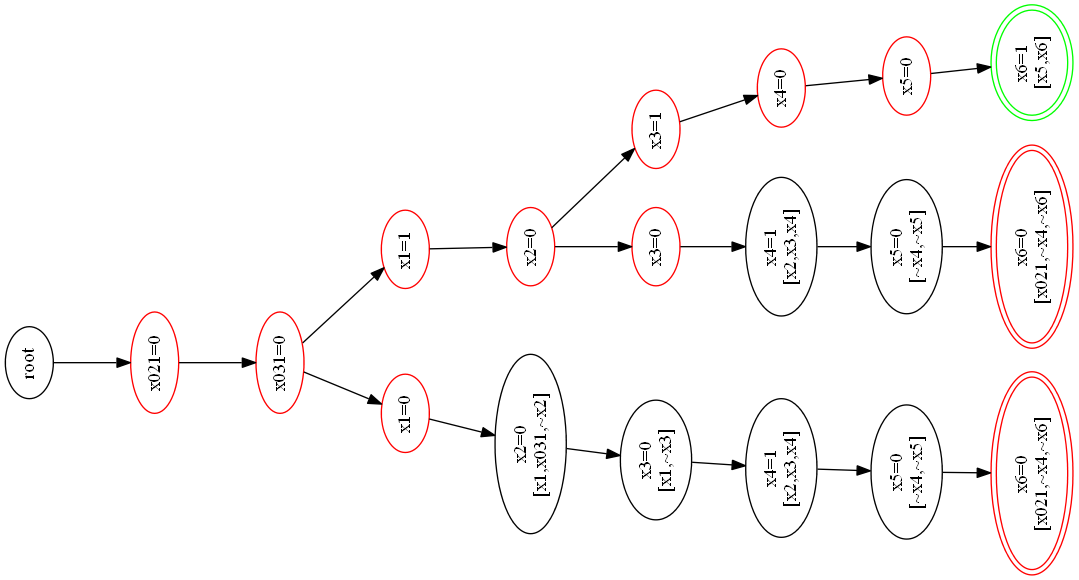
\includegraphics[keepaspectratio=true,height=.7\textheight]{tree1}
\end{center}

\vfill

\newpage

\section{Configuration}

\p{config.pro} contains: the default algorithmic mode, the default
display options, and the \dt{} prologue and decorations. The predicate
\p{decorate\_mode} determines which family of decorations will be used.

\p{show\_config} displays: the version and copyright notice, the
defaults from \p{config.pro}, changes from the default values, and the
variable order.


\section{Test programs included in \ls{}}

\begin{itemize}
\item \p{examples.pro}: Examples from papers on SAT
solvers \cite{mz,mlm,ms}.

\item \p{tseitin.pro}: Tseitin clauses for $K_{2,2}$,
$K_{3,3}$ and the example from \cite[Section 4.5]{mlcs}.

\item \p{queens.pro}: The 4-queens problem.

\item \p{pigeon.pro}: The pigeonhole principle for 2 and 3 holes.

\item \p{pebbles.pro}: Grid pebbling for 2 and 3 layers.
\end{itemize}

\section{DIMACS transformation}

The predicates in \p{dimacs.pro} convert a set of clauses in
\pl{} format (a list of lists of literals) to and from \emph{DIMACS cnf
format}:
\begin{itemize}
\item \p{to\_dimacs(File, Comment, Clauses)} converts the \pl{}
\p{Clauses} into DIMACS format and writes them to the \p{File} with the
\p{Comment}.
\item \p{from\_dimacs(Predicate, InFile, OutFile)} reads \p{InFile} in
DIMACS format and writes a \pl{} program to \p{OutFile} as
\verb+Predicate :- dpll(List, _).+
\end{itemize}

\section{Portability}\label{s.port}

\ls{} was developed on \sw{} but an effort was made to use only portable
constructs. The possible exceptions are:

\begin{itemize}
\item Modules: \p{module}, \p{use\_module}, \p{reexport}.
\item The following predicate to obtain the file name from the command
line:
\begin{verbatim}
current_prolog_flag(argv, [_, File | _])
\end{verbatim}
\end{itemize}

\newpage


\section{Module structure}

The \ls{} software consists of the following source files (not including
the test programs and the program for DIMACS conversion):

\begin{itemize}
\item \p{dpll.pro}: Main module for the DPLL algorithms.

\item \p{cdcl.pro}: Algorithms for CDCL and the implication graph.

\item \p{auxpred.pro}: Auxiliary predicates for the algorithms. 

\item \p{io.pro}: Predicates for writing assignments, clauses and
implication graphs.

\item \p{display.pro}: Display the trace using predicates \p{display/n},
where the first argument is a display option and the additional
arguments supply the data to be displayed.

\item \p{config.pro}: Default configuration data.

\item \p{counters.pro}: Maintains and displays counters for units,
decisions and conflicts. Stores the number of clauses and variables for
printing the statistics. Defines counters for adding a number to the
file names for implication graphs and trees of assignments.

\item \p{modes.pro}: Sets, clears and checks the mode and the display
options. Implements \p{usage} and \p{show\_config}. The dummy
display option \p{none} is used to distinguish between the initial state
(no options, so set the default options) and a state where all options
have been cleared.

\item \p{dot.pro}: Generate the \dt{} files of the implication graphs
and the assignment trees.
\end{itemize}

\section{Data structures}

The following dynamic predicates are used:
\begin{itemize}
\item In \p{cdcl.pro}: The non-chronological backtracking level in the
predicate \p{backtrack}.

\item In \p{cdcl.pro}: The learned clauses are stored as a list of
clauses in the predicate \p{learned}.

\item In \p{auxpred.pro}: If the user specifies the order of assignment
to variables, the list is stored in \p{variables\_list}.

\item In \p{dot.pro}: \p{node} and \p{edge} are used when building the
assignment trees. They store the paths leading to previous conflict
nodes and are updated with each new path.

\item In \p{mode.pro}: The current mode \p{alg\_mode} and display
options \p{display\_option}. 

\end{itemize}

\newpage

Two functors are used to create terms:
\begin{itemize}

\item \p{assign} represents an assignment and takes four arguments: a
variable, its value, its level and either \p{yes} if this is a decision
assignment or the antecedent clause of an implied assignment.

\item \p{graph} is an implication graph. Its arguments are a list of
nodes which are assignments and a list of edges which are terms with
functor \p{edge} and three arguments: the source and target nodes
and the clause that labels the edge.
\end{itemize}


\section{The DPLL algorithm}

The predicate \p{dpll/2} implements the DPLL algorithm on a set of
clauses represented as a list of lists of literals. It returns a list of
satisfying assignments or the empty list if the clauses are
unsatisfiable. As part of its initialization, the set of variables in
the clauses is obtained from the list.

The predicate \p{dpll/2} invokes \p{dpll/6} which is the main recursive
predicate for performing the algorithm. If the set of variables to be
assigned to is empty, the set of clauses is satisfiable. Otherwise,
\p{dpll/6} tries to perform unit propagation by searching for a unit and
then evaluating the set of clauses. When no more units remain, it
chooses a decision assignment and evaluates the set of clauses.

The predicate \p{ok\_or\_conflict} is called with the result of the
evaluation of unit propagation or the choice of an assignment. If the
result is not a conflict, the variable chosen is deleted and \p{dpll/6}
is called recursively. If there was a conflict, the implication graph is
constructed and a learned clause is generated from the graph; then
\p{ok\_or\_conflict} fails so that backtracking can try a new
assignment.

The predicate \p{evaluate} receives a set of clauses and evaluates them,
returning \p{ok} or \p{conflict}. For each clause it calls
\p{evaluate\_clause}, which returns \p{satisfied}, \p{unsatisfied},
\p{unit} or \p{unresolved}.

\p{find\_unit} traverses the list of clauses using the current
assignments. It calls \p{evaluate\_clause} on each clause and succeeds
if that predicate returns \p{unit}.

\p{choose\_assignment} returns an assignment. A conditional construct
with an internal cut-fail implements non-chronological backtracing. (See
Section~4.7 of the \sw{} Reference Manual.)


\section{CDCL and NCB}

The implication graph is built incrementally. Whenever a unit clause is
found, \p{extend\_graph} is called with the unit clause, its number (to
label the new edges), the assignment it implies (to create the new
target of the edges) and the graph constructed so far. For each literal
(except the one implied), a new edge is created and when the list of
literals has been traversed, the new node is created. When a conflict is
encountered, the \p{kappa} node and its incoming edges are added.
Two predicates for computing a learned clause are now called.

\p{compute\_learned\_clause\_by\_dominator} locates a dominator of the
highest-level decision assignment node relative to the \p{kappa} node.
The predicate \p{findall} is frequently used but is encapsulated in
other predicates. \p{get\_paths\_to\_kappa} returns a list of all paths
from the decision node to the \p{kappa} node. This list is an argument
to \p{get\_dominator} which finds a node that appears on all the paths.
\p{get\_paths\_to\_kappa} is called again to find paths from decision
assignments at \textit{lower} levels to \p{kappa} and then paths that go
through the dominator are removed. From the remaining paths, edges are
located that go from nodes of lower level to nodes of the highest level.
The complements of the assignments at the source nodes of these edges,
together with the complement of the assignment at the dominator, define
the learned clause.

\p{compute\_learned\_clause\_by\_resolution} starts with the conflict
clause (the antecedent clause of the \p{kappa} node) as the current
clause. \p{learn\_clause\_from\_antecedents} uses the list of
assignments so far to locate the antecedent of the assignment associated
with the current clause. \p{resolve} resolves the two clauses and
\p{learn\_clause\_from\_antecedents} is called with the resolvent as the
new current clause. The algorithm terminates when \p{check\_uip}
identifies the current clause as a UIP and this clause becomes the
learned clause.

\emph{The clause learned by resolution is added to the list of learned
clauses in the dynamic predicate \p{learned}.}

\p{compute\_backtrack\_level} returns the highest level of an assignment
in the learned clause except for the current level.


\section{Auxiliary predicates}\label{s.aux}

\begin{itemize}

\item \p{is\_assigned} checks if a literal has been assigned a value
and if so returns that value.

\item \p{literals\_to\_variables} takes a list of literals and returns a
sorted set of the variables corresponding to the literals.

\item \p{to\_variable} returns the variable of a literal;
\p{to\_complement} returns the complement of a literal.

\item \p{to\_assignment} and \p{to\_literal} convert to and from a
literal and an assignment expressed as a term \p{assign(Variable, Value,
Level, Decision)}.

\end{itemize}


\bibliographystyle{plain}
\bibliography{learnsat}
\end{document}
